%%%%%%%%%%%%%%%%%%%%%%%%%%%%%%%%%%%%%%%%%%%%%%%%%%%%%%%%%%%%%%%%%%%%%%%%%%%%%%%

\chapter{METODOLOGIA DE FOURIER}

Análise de Fourier é uma coleção de técnicas para representar funções (ou sinais) gerais como a combinação linear de funções periódicas \cite{li1999fourier}. As ferramentas mais úteis na análise de Fourier são as três transformadas: Séries de Fourier, Transformada Discreta de Fourier (DFT) e Transformada Contínua de Fourier. O processo de calcular as transformadas é chamado de Análise Espectral de Fourier, e esta será a técnica aqui explorada para analisar os dados introduzidos na seção anterior.

Séries de Fourier são úteis para representar funções reais periódicas como uma soma de senos e cossenos com seus respectivos coeficientes (ou pesos). Tais funções sinusoidais formam uma base ortogonal no Espaço de Fourier. As Figuras \ref{fig:FSsqw} e \ref{fig:FSx} ilustram a representação de sinais via Séries de Fourier.

%\vspace{-7mm}
\begin{figure}[ht!]
	\caption{Exemplo Série de Fourier - função periódica.}
	\vspace{1mm}	% acrescentar o espaçamento vertical apropriado entre o título e a borda superior da figura
	\begin{center}
		\resizebox{9cm}{!}{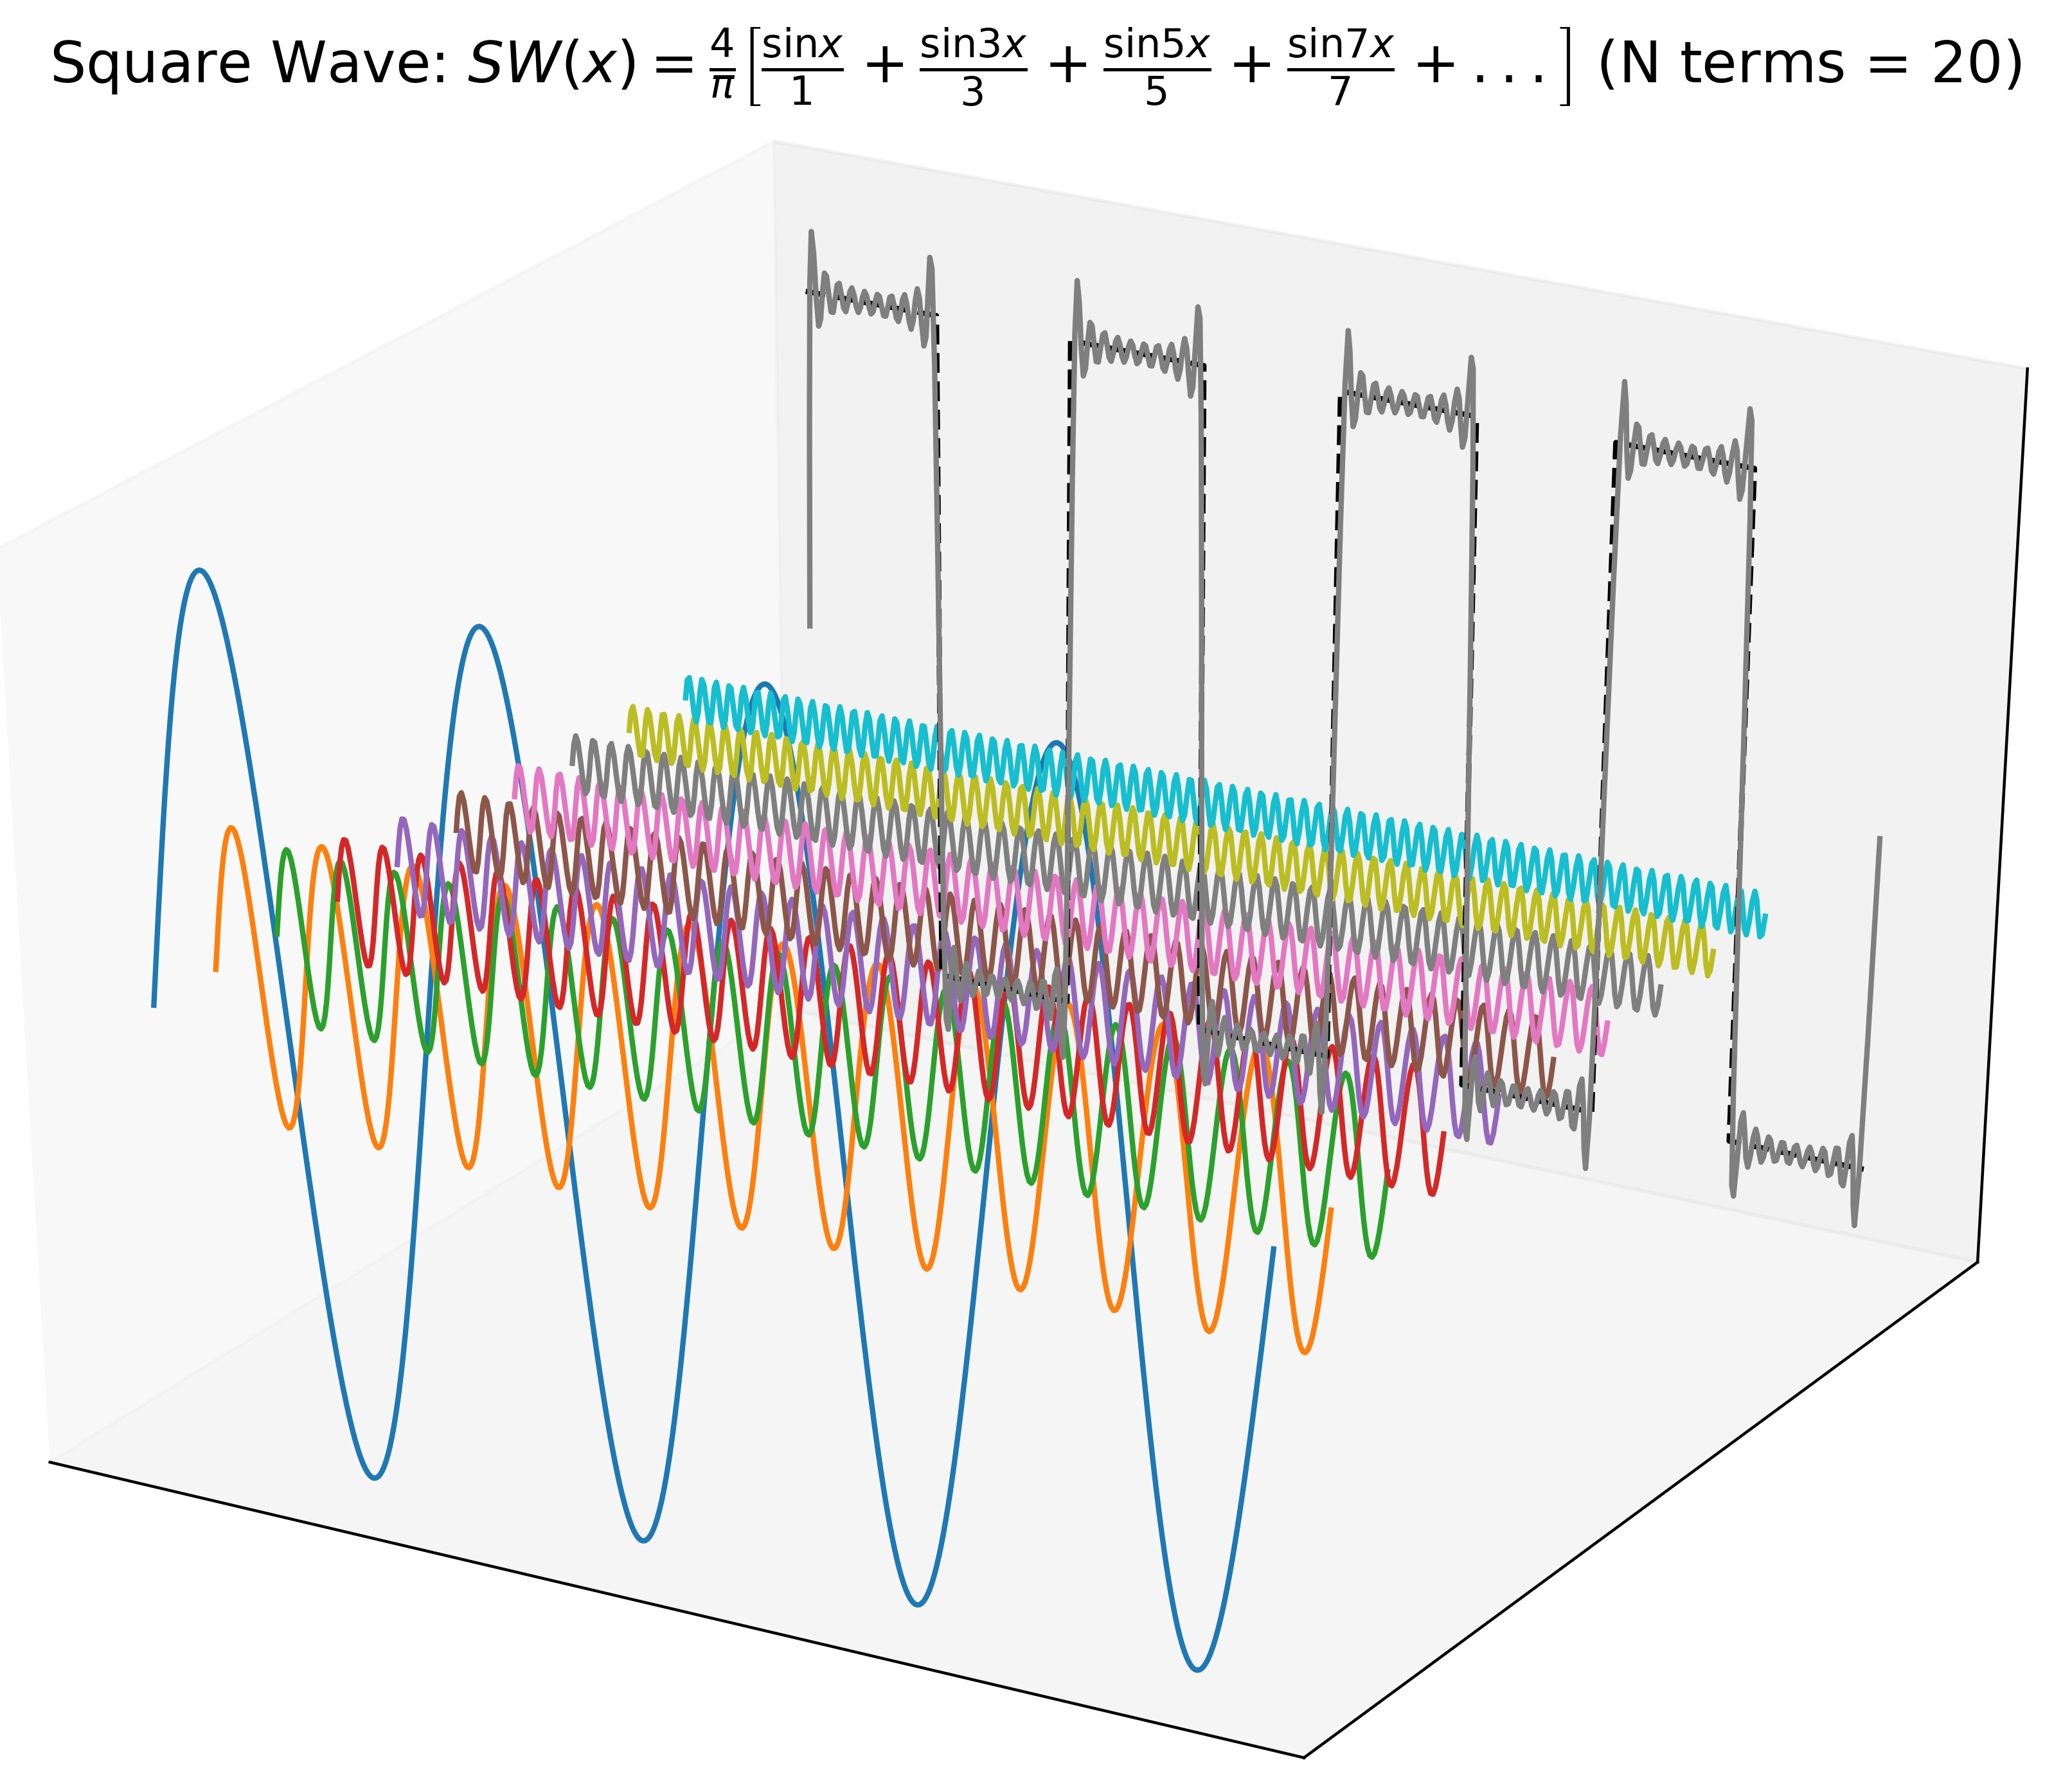
\includegraphics{Figuras/sqw.jpg}}
	\end{center}
	\vspace{0mm}	% acrescentar o espaçamento vertical apropriado entre a borda inferior da figura e a legenda ou a fonte quando não há legenda (o valor pode ser negativo para subir)
	\legenda{Representação de um sinal de perfil quadrado (linha tracejada preta ao fundo) como a soma de senos (linha cinza cheia sobre a linha preta tracejada). No gráfico, os vinte primeiros termos da série são apresentados em sequência.}	% legenda - para deixar sem legenda usar comando \legenda{} (nunca deve-se comentar o comando \legenda)
	\label{fig:FSsqw}
	%\FONTE{\url{https://omniweb.gsfc.nasa.gov/form/dx1.html}.}	% fonte consultada (elemento obrigatório, mesmo que seja produção do próprio autor)
\end{figure}
%\vspace{-12mm}
\begin{figure}[ht!]
	\caption{Exemplo Série de Fourier - função não periódica.}
	\vspace{1mm}	% acrescentar o espaçamento vertical apropriado entre o título e a borda superior da figura
	\begin{center}
		\resizebox{9cm}{!}{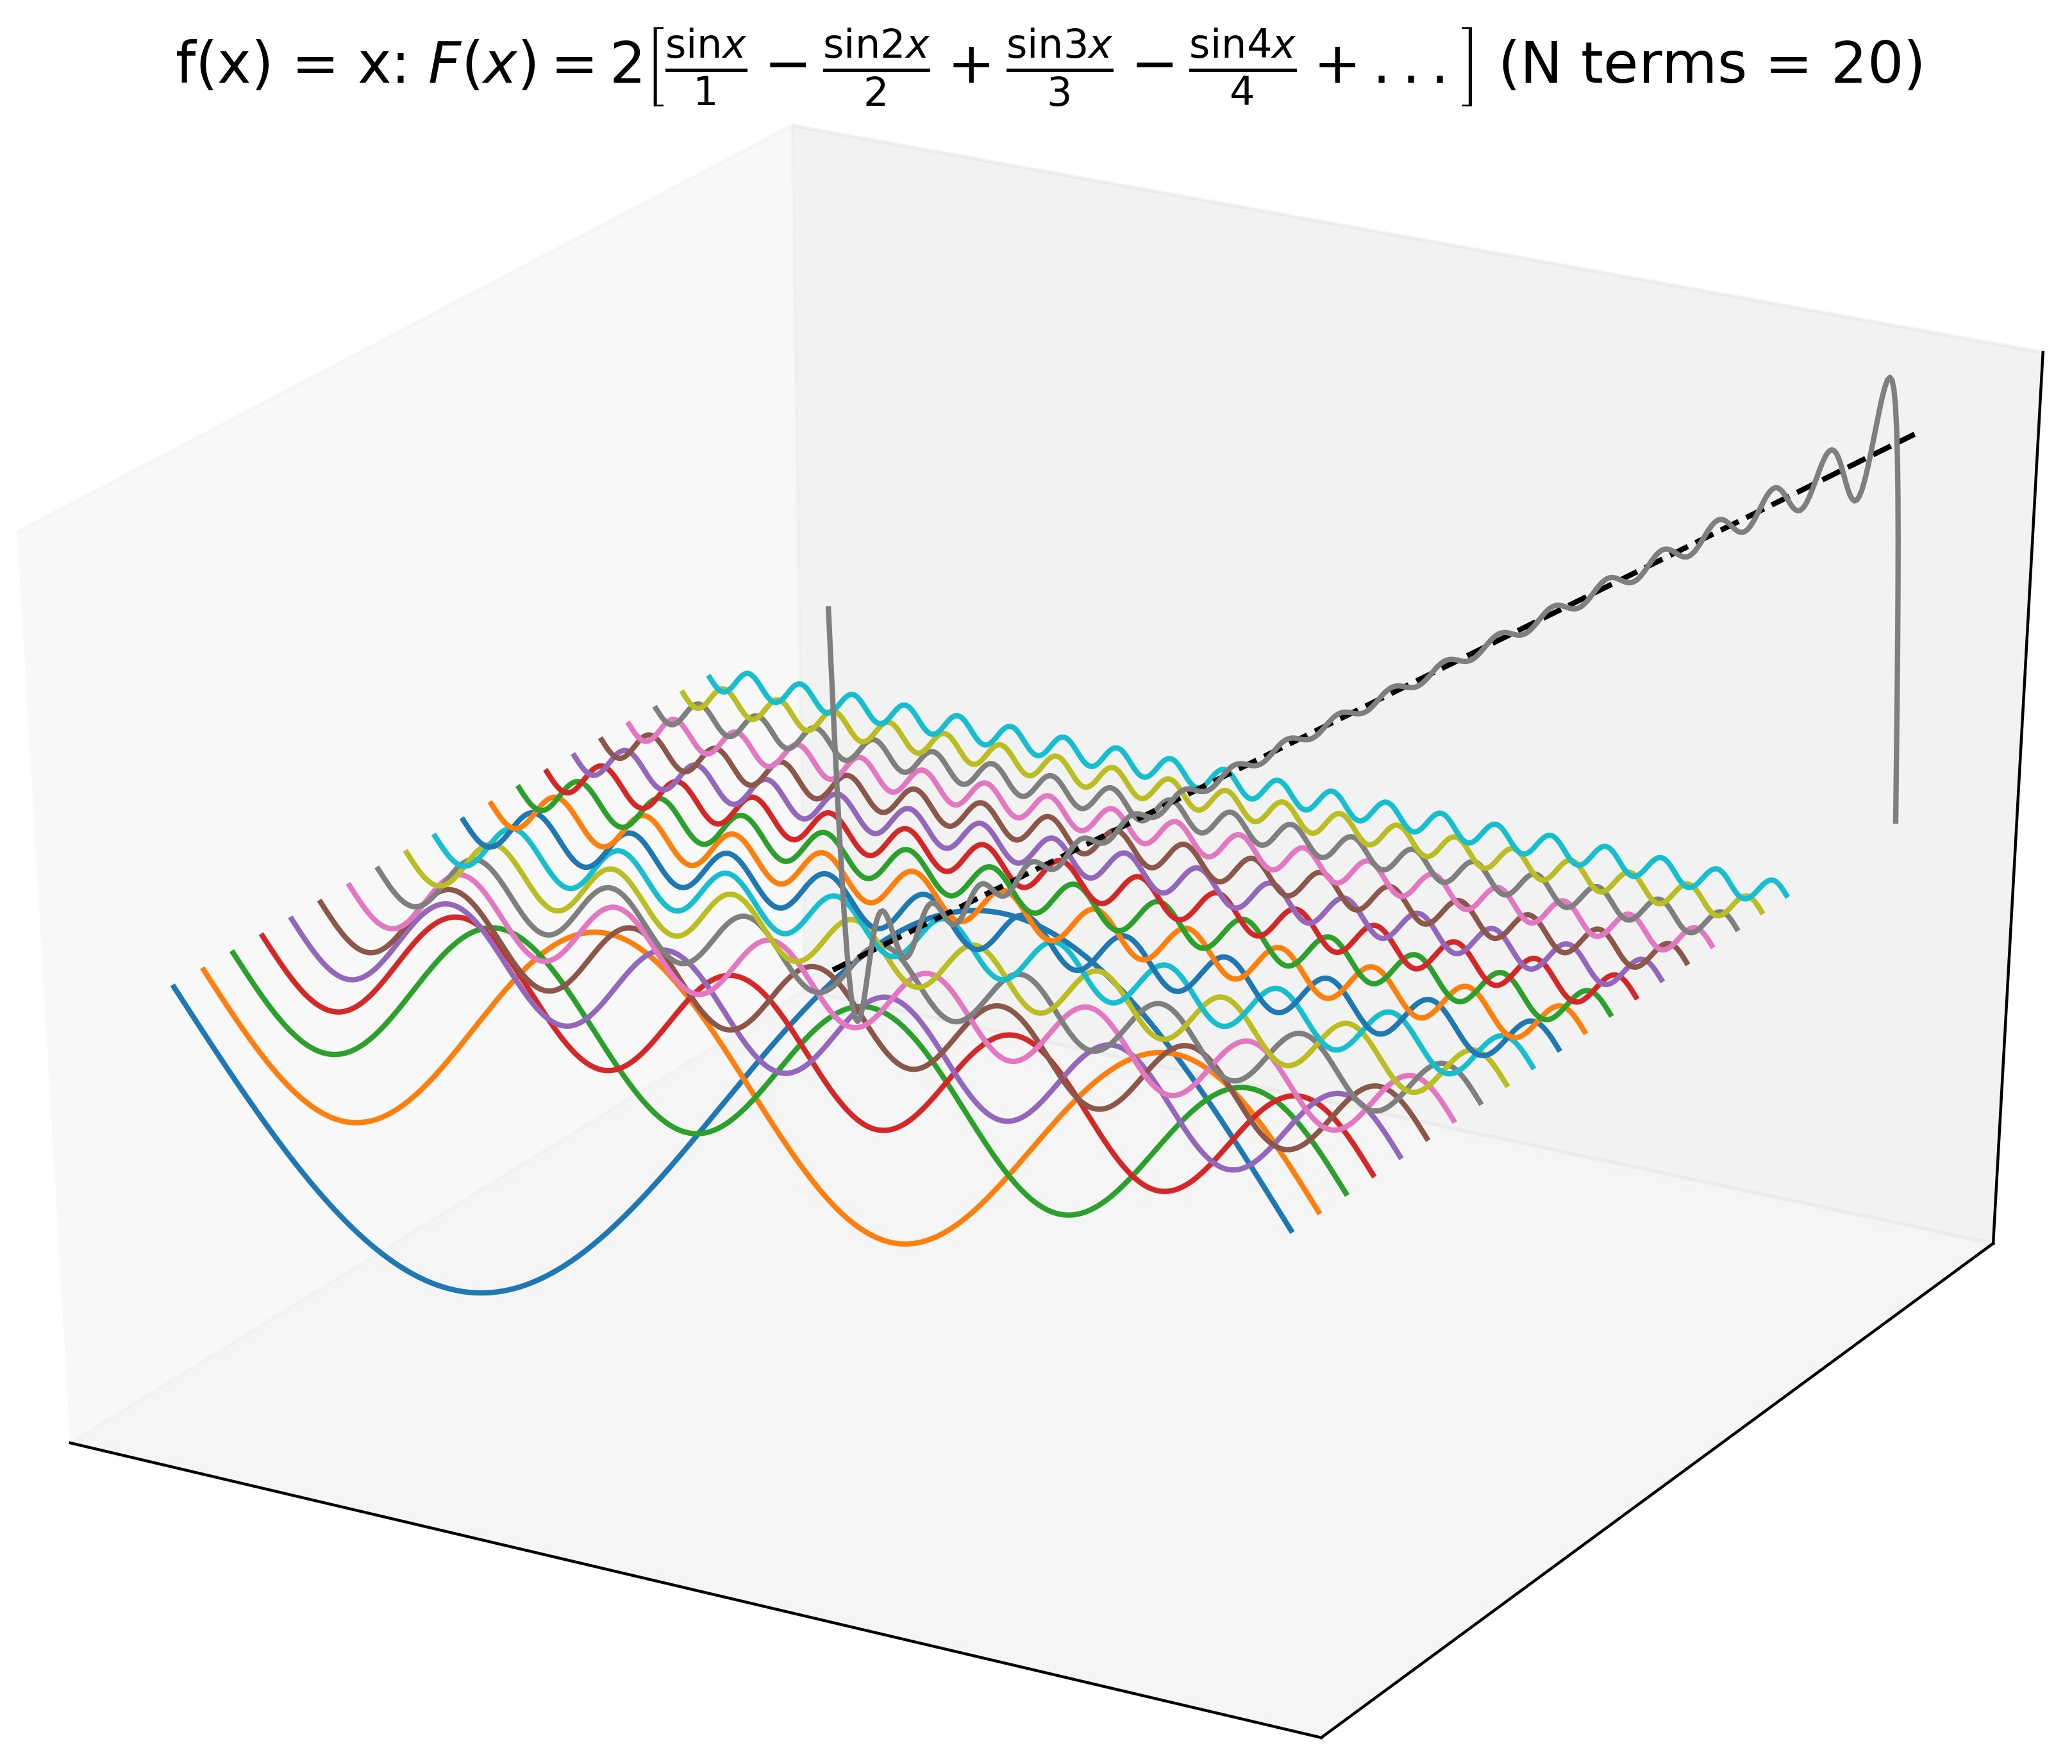
\includegraphics{Figuras/x.jpg}}
	\end{center}
	\vspace{0mm}	% acrescentar o espaçamento vertical apropriado entre a borda inferior da figura e a legenda ou a fonte quando não há legenda (o valor pode ser negativo para subir)
	\legenda{Aplicação das Séries de Fourier, desta vez sobre a função $f(x)= x $. Pode-se observar que mesmo para uma função não necessariamente periódica, é possível a representação em termos de funções sinusoidais. Os vinte primeiros termos foram usados para representar a função.}	% legenda - para deixar sem legenda usar comando \legenda{} (nunca deve-se comentar o comando \legenda)
	\label{fig:FSx}
	%\FONTE{\url{https://omniweb.gsfc.nasa.gov/form/dx1.html}.}	% fonte consultada (elemento obrigatório, mesmo que seja produção do próprio autor)
\end{figure}

A Transformada de Fourier (ou FT, uma abreviação do inglês \textit{Fourier Transform}) não requer que um sinal seja periódico para ser utilizada. Entretanto, ela intrinsecamente considera que o sinal é uma composição de ondas senoidais (bem localizadas na frequência e mal localizadas no tempo). A FT pode ser usada para analisar os conteúdos frequenciais de um sinal, e assim investigar persistências da série. 

Uma aplicação da FT é o chamado espectro de potência. Ele é definido como o módulo quadrado da FT. Ele representa a energia associada a cada conteúdo frequencial. Em outras palavras, a contribuição de cada frequência para a energia total do sinal. A Figura \ref{fig:FT_exemplo} é um exemplo do espectro de potência calculado para os sinais $f_{1}$, $f_{2}$ e uma combinação destes, evidenciando o significado do seu resultado, bem como a característica linear da FT.

\begin{figure}[ht!]
	\caption{Exemplo Transformada de Fourier.}
	\vspace{1mm}	% acrescentar o espaçamento vertical apropriado entre o título e a borda superior da figura
	\begin{center}
		\resizebox{15cm}{!}{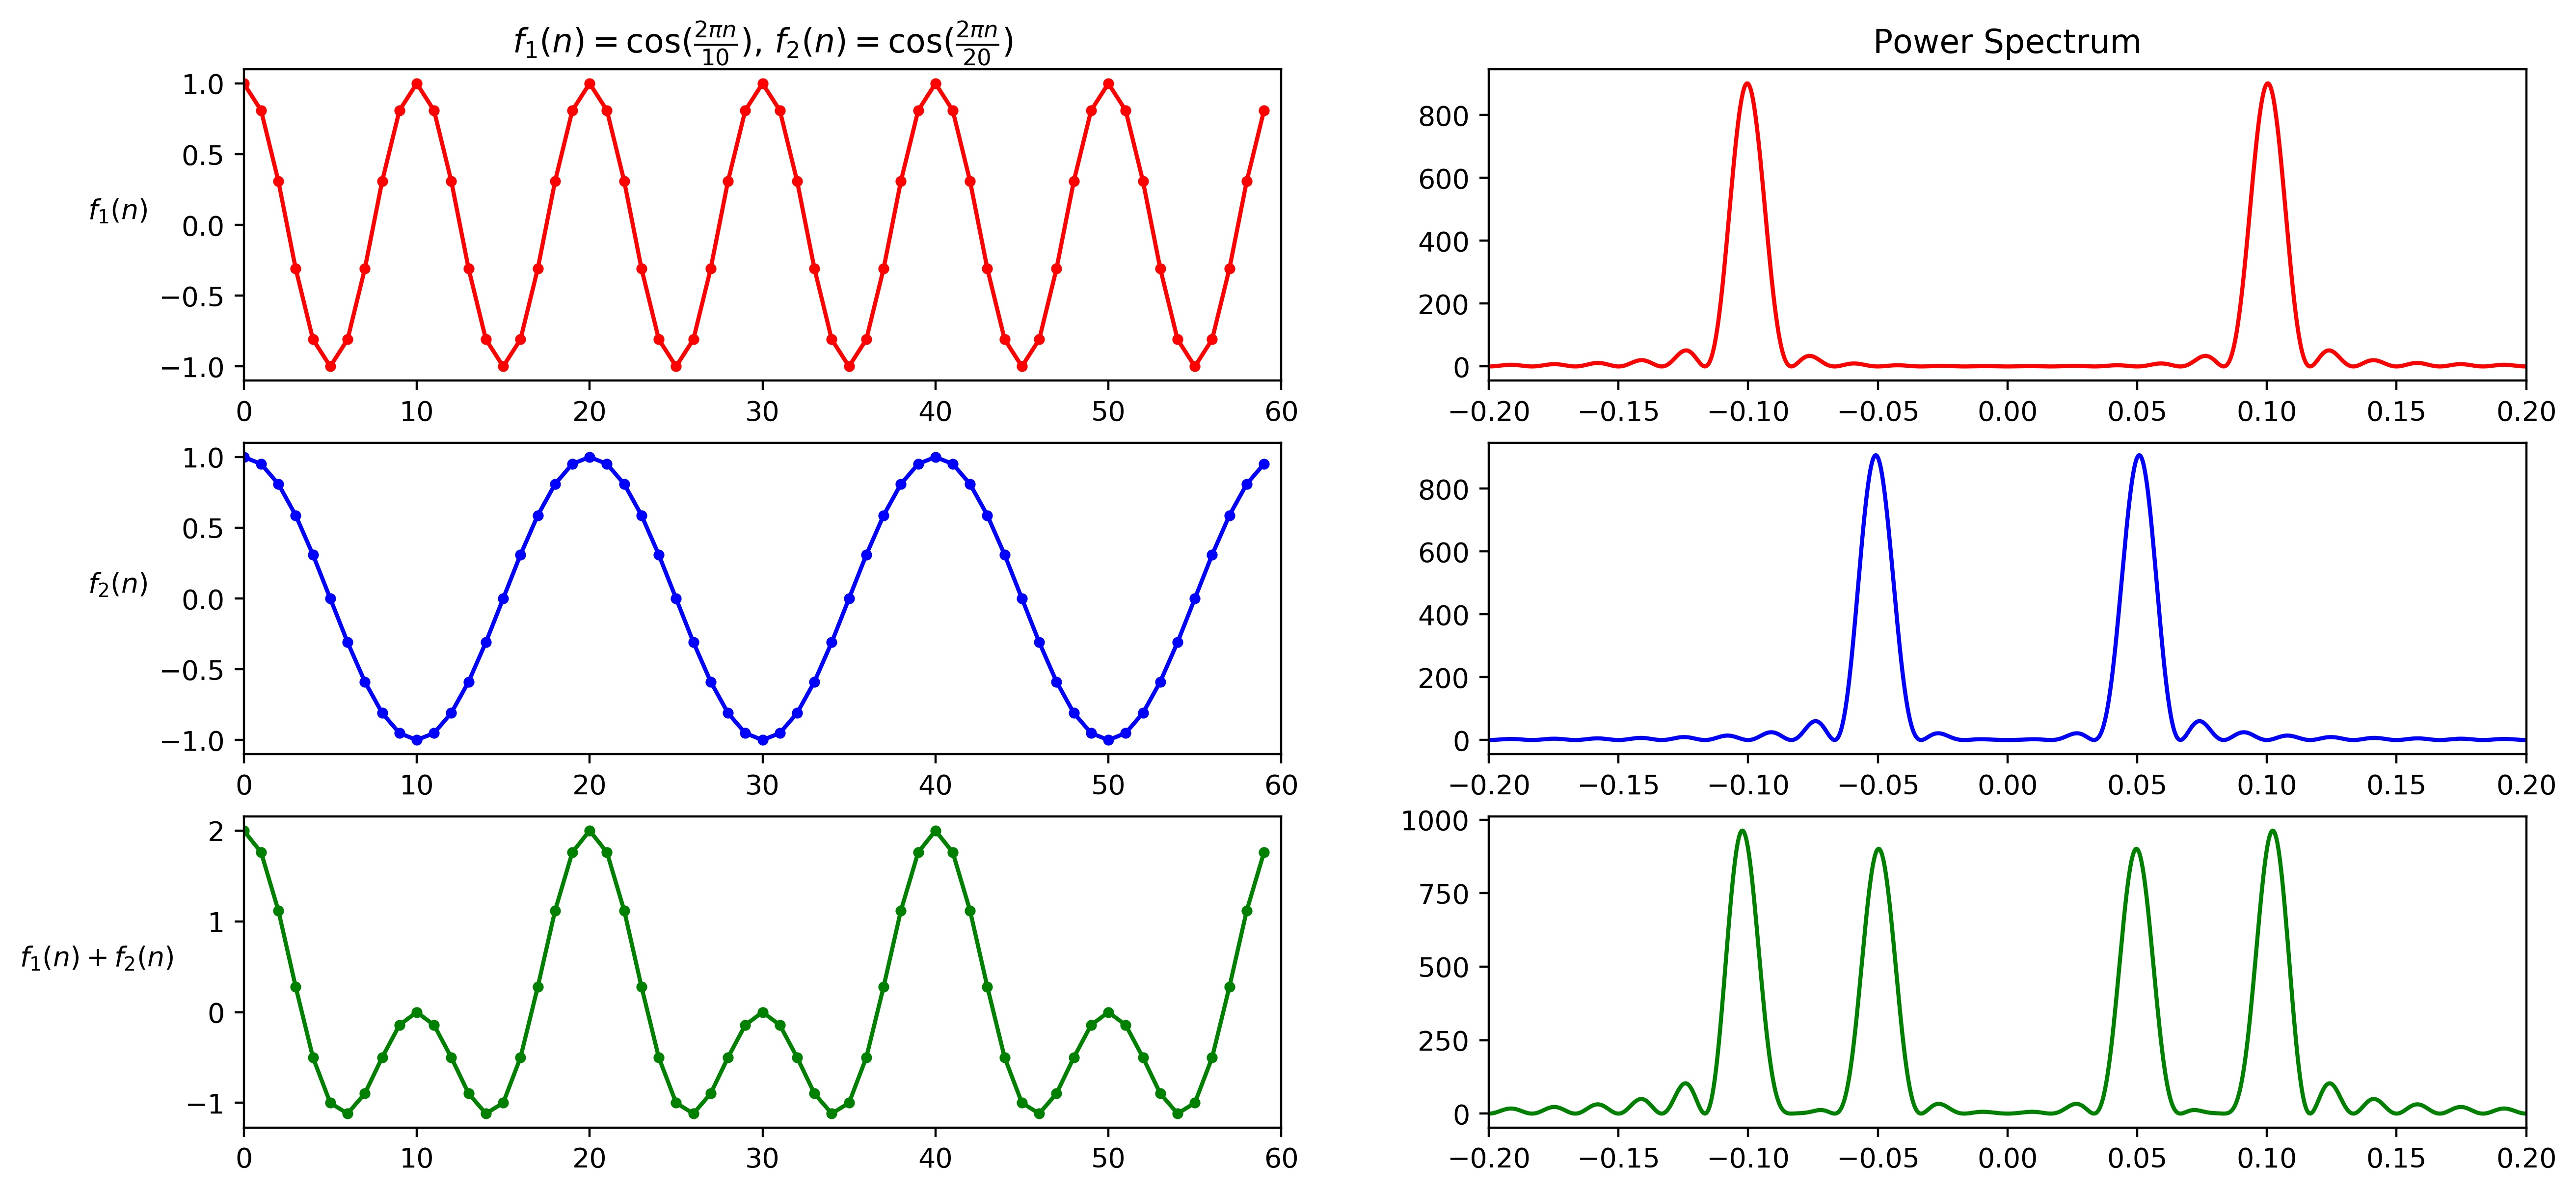
\includegraphics{Figuras/ft_exemplo.jpg}}
	\end{center}
	\vspace{1mm}	% acrescentar o espaçamento vertical apropriado entre a borda inferior da figura e a legenda ou a fonte quando não há legenda (o valor pode ser negativo para subir)
	\legenda{Esquerda: funções $f_{1}$ (no topo, de frequência 0.1), $f_{2}$ (no meio, de frequência 0.5) e uma combinação destas (abaixo). Direita: espectro de potência dos respectivos sinais à esquerda. O último plot evidencia a característica linear da FT, onde a soma dos sinais resultou num espectro de potência com duas assinaturas de frequência, correspondentes às assinaturas individuais dos sinais $f_{1}$ e $f_{2}$.}	% legenda - para deixar sem legenda usar comando \legenda{} (nunca deve-se comentar o comando \legenda)
	\label{fig:FT_exemplo}
	%\FONTE{\url{https://omniweb.gsfc.nasa.gov/form/dx1.html}.}	% fonte consultada (elemento obrigatório, mesmo que seja produção do próprio autor)
\end{figure}

Para a análise espectral dos dados de F10.7, foi utilizada a biblioteca \texttt{Numpy} do \texttt{Python}, com a rotina \texttt{fft} para computar a Transformada Discreta de Fourier. Baseada no algoritmo FFT (Fast Fourier  Transform), ela explora a simetria dos termos calculados e computa a DFT de forma eficiente \cite{cooley1965algorithm}. Conforme o manual, a função \texttt{numpy.fft.fft}, particularmente utilizada  nesta análise, fornece a transformada não normalizda. Se \texttt{A = fft(input)}, o primeiro termo do output \texttt{A[0]} é o de frequência zero, ou seja, a soma do sinal. \texttt{A[1:n/2]} contém os termos de frequência positiva e \texttt{A[n/2+1:]} contém os termos de frequência negativa. O espectro de potência é obtido fazendo-se \texttt{numpy.abs(A)**2}. Tais informações foram usadas para gerar a Figura \ref{fig:FT_exemplo} e também os resultados apresentados na próxima seção.
